\documentclass[tikz,border=8pt]{standalone}
\usepackage{amsmath,amssymb}
\usetikzlibrary{arrows.meta,calc}

\begin{document}
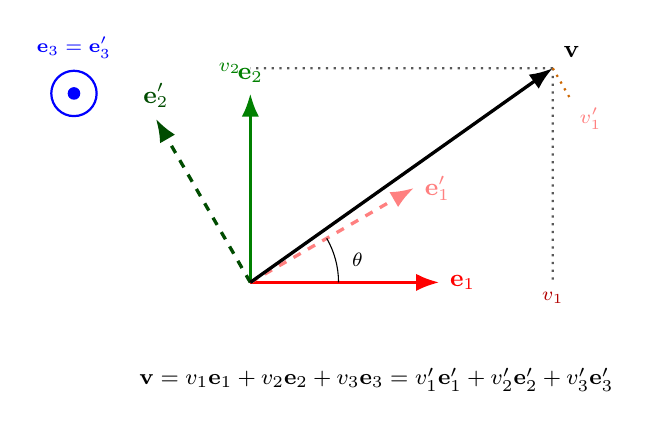
\begin{tikzpicture}[>=Latex, scale=1.6]

  % Standard basis
  \draw[->, red, very thick] (0,0) -- (1.5, 0) node[right, font=\small]{$\mathbf e_1$};
  \draw[->, green!50!black, very thick] (0,0) -- (0, 1.5) node[above, font=\small]{$\mathbf e_2$};

  % Rotated basis at 30 deg (dashed lighter)
  \draw[->, red!50, very thick, dashed] (0,0) -- ({1.5*cos(30)},{1.5*sin(30)}) node[right, font=\small]{$\mathbf e'_1$};
  \draw[->, green!30!black, very thick, dashed] (0,0) -- ({-1.5*sin(30)},{1.5*cos(30)}) node[above, font=\small]{$\mathbf e'_2$};

  % Rotation arc
  \draw[thin] (0.7, 0) arc (0:30:0.7);
  \node[font=\scriptsize] at (0.85, 0.18) {$\theta$};

  % Vector v
  \coordinate (v) at (2.4, 1.7);
  \draw[->, black, very thick] (0,0) -- (v) node[above right, font=\small]{$\mathbf v$};

  % Standard projections
  \draw[dotted, thick, gray!70!black] (v) -- (2.4, 0);
  \draw[dotted, thick, gray!70!black] (v) -- (0, 1.7);
  \node[below, font=\scriptsize, red!70!black] at (2.4, 0) {$v_1$};
  \node[left, font=\scriptsize, green!50!black] at (0, 1.7) {$v_2$};

  % Rotated projections
  \pgfmathsetmacro{\vp}{2.4*cos(30) + 1.7*sin(30)}
  \pgfmathsetmacro{\px}{\vp*cos(30)}
  \pgfmathsetmacro{\py}{\vp*sin(30)}
  \draw[dotted, thick, orange!80!black] (v) -- (\px, \py);
  \node[below right, font=\scriptsize, red!50] at (\px, \py) {$v'_1$};

  % e3 fixed (out of page)
  \draw[blue, thick] (-1.4, 1.5) circle (0.18);
  \fill[blue] (-1.4, 1.5) circle (0.05);
  \node[font=\scriptsize, blue, anchor=south] at (-1.4, 1.7) {$\mathbf e_3=\mathbf e'_3$};

  % equation
  \node[align=center, font=\footnotesize, anchor=north] at (1.0, -0.6)
    {$\mathbf v=v_1\mathbf e_1+v_2\mathbf e_2+v_3\mathbf e_3=v'_1\mathbf e'_1+v'_2\mathbf e'_2+v'_3\mathbf e'_3$};
\end{tikzpicture}
\end{document}
